\documentclass[10pt]{article}
\usepackage[margin=0.65in]{geometry}
\usepackage[T1]{fontenc}
\usepackage{lmodern,graphicx,amsmath,hyperref}
\hypersetup{colorlinks=true,urlcolor=blue}
\setlength{\parindent}{0pt}
\setlength{\parskip}{5pt}
\title{APS measurement instrument: implementation and open gates}
\author{Native ecbench continuation}
\date{30 October 2026}
\begin{document}
\maketitle
\textbf{Outcome and scope.} This adds a bounded native ecbench adapter for the
four existing APS solver/encoding leads. It is instrumentation, not a measured
improvement. No performance experiment has launched. Practical speed, scaling,
complete operation cost and the full research panel remain unresolved.

\textbf{What is charged.} One monotonic timeline records target-independent
setup, then all target-dependent work: validation and labeled-base sampling,
polynomial construction and equation-export binding, F4 and root extraction,
signed checks, modular recovery and independent affine verification. Setup plus
the five exclusive online phases equals the cold solver interval exactly.
All retries, pre-transcript aborts, failed branches and deadlines remain in the
record. Final report aggregation/serialization is outside the algorithm interval; observer
and equation-export construction overhead is inside and must be assessed.

\begin{center}
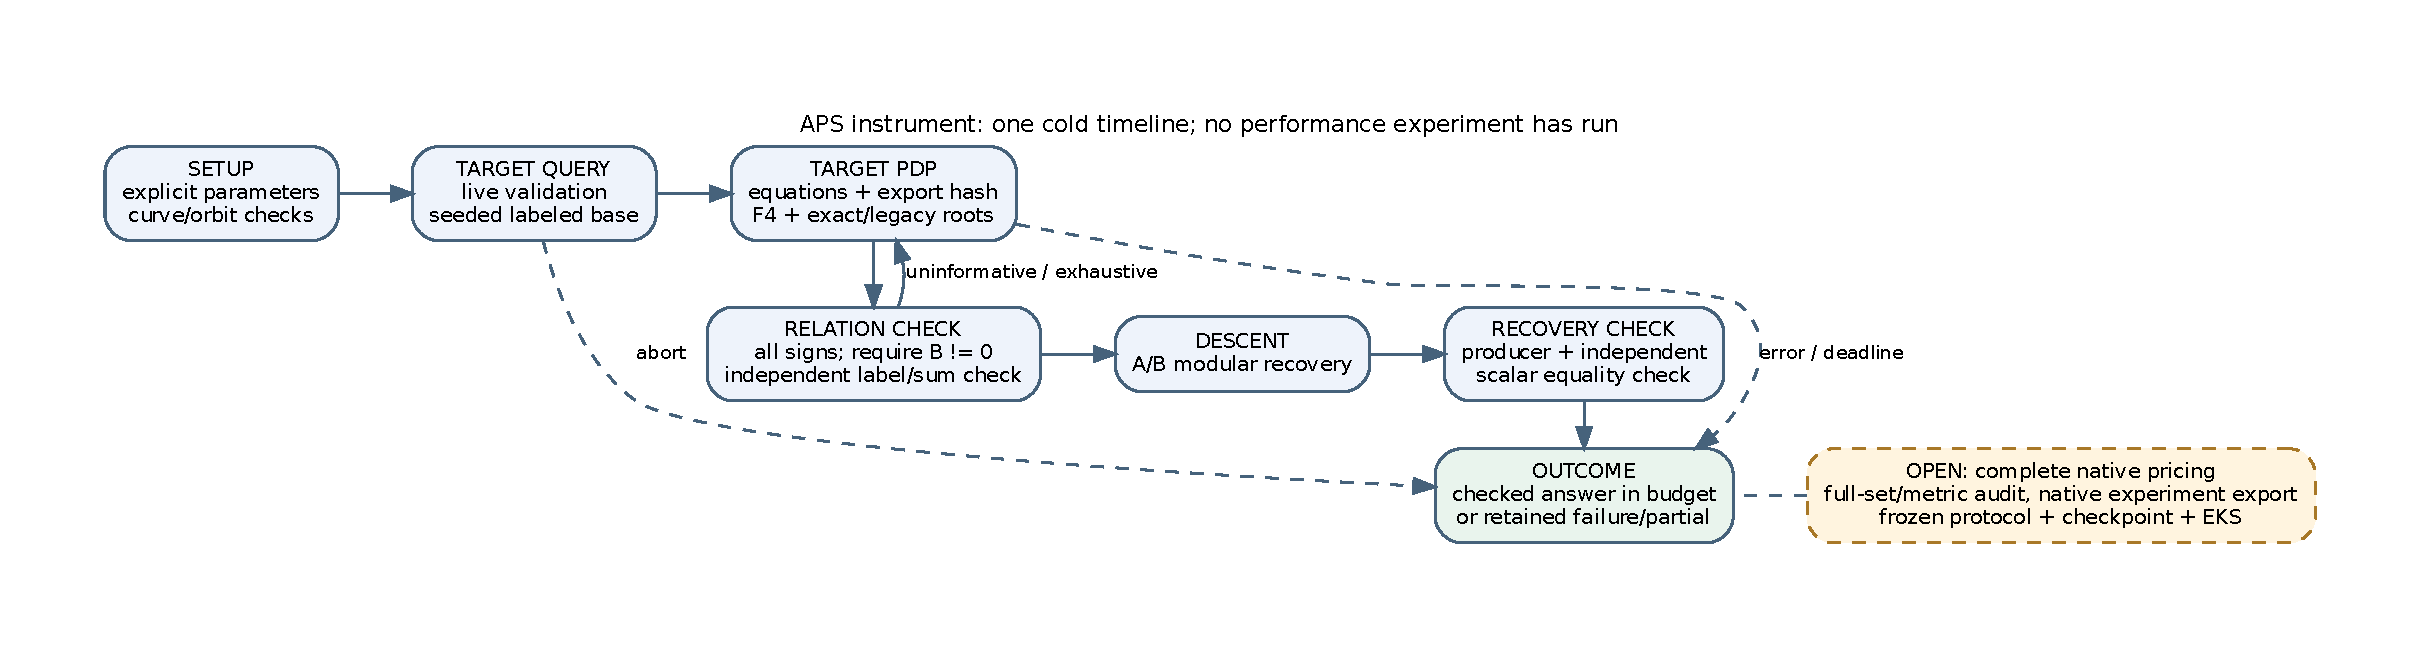
\includegraphics[width=\linewidth]{instrument.pdf}
\end{center}

\textbf{Controls and correctness.} Search parameters are explicit. The same
constructor and seed support exhaustive/first-informative, legacy/exact roots,
unordered cubic/line divisor and certified orbit line/pruning controls.
Unsupported combinations are refused at planning. Every accepted witness is
checked with separate ordinary-residue affine arithmetic: its labels, signed
zero sum, nonzero denominator, modular equation and final scalar recovery.
This attests a witness, not root completeness, execution history or costs.

\textbf{Native-accounting limit.} F4/root multiplication diagnostics and the
independent check's group operations are retained. Core group/field work,
polynomial construction, allocation and hashing are not completely counted or
priced. GAE is consequently a lower bound; complete S and bitop/v1 rankings
are inadmissible. The native-work-complete, cost-attested and independently
complete-set-audited flags remain false. Closing a wall interval does not
close this operation ledger.

\textbf{Next evidence.} Review a held-out four-size ladder within the existing
prime-field bound, complete the native unified export and metric/full-output
validation, and freeze the schema-valid protocol, controls, seeds, analysis,
sample-size rationale and budget before affected data. EKS admission requires
L2, A/A, verified source/image/binary identities and the applicable recovery
contract. The mandatory source checkpoint is still blocked by the earlier
explicit upload rejection; no alternate route or smaller upload evades it.

\textbf{Sources and validation.} The source-linked README, CHECKS and protocol
draft accompany this report; final normalized receipts pin the code actually
checked. Prior studies retain their original validation boundaries. This adds
no theorem or Lean claim, paper-scale reproduction, new curve route or
security conclusion. Development-test durations are not performance evidence.

\small
\href{https://github.com/isogeny-labs/crypto/blob/3d504e2062016046f854307a82e1026df199cbd6/src/cryptanalysis/ecbench/aps/mod.rs}{Native adapter};
\href{https://github.com/isogeny-labs/crypto/blob/3d504e2062016046f854307a82e1026df199cbd6/src/cryptanalysis/aps_single_relation.rs}{existing APS solver and observers};
\href{https://github.com/isogeny-labs/crypto/blob/main/research/aps_followup_20261028/README.md}{APS manuscript/source map};
\href{https://www.secg.org/sec1-v2.pdf}{SEC 1 v2.0, sections 2.2.1/3.2.2.1};
\href{https://github.com/isogeny-labs/crypto/blob/main/docs/ecbench/README.md}{ecbench standard}.
\end{document}
